\newpage
    \subsection{Task 2.2: Sequence diagrams}
    \subsubsection{Request For Printing Service}
    \begin{center}
    \begin{figure}[!htp]
    \begin{center}
     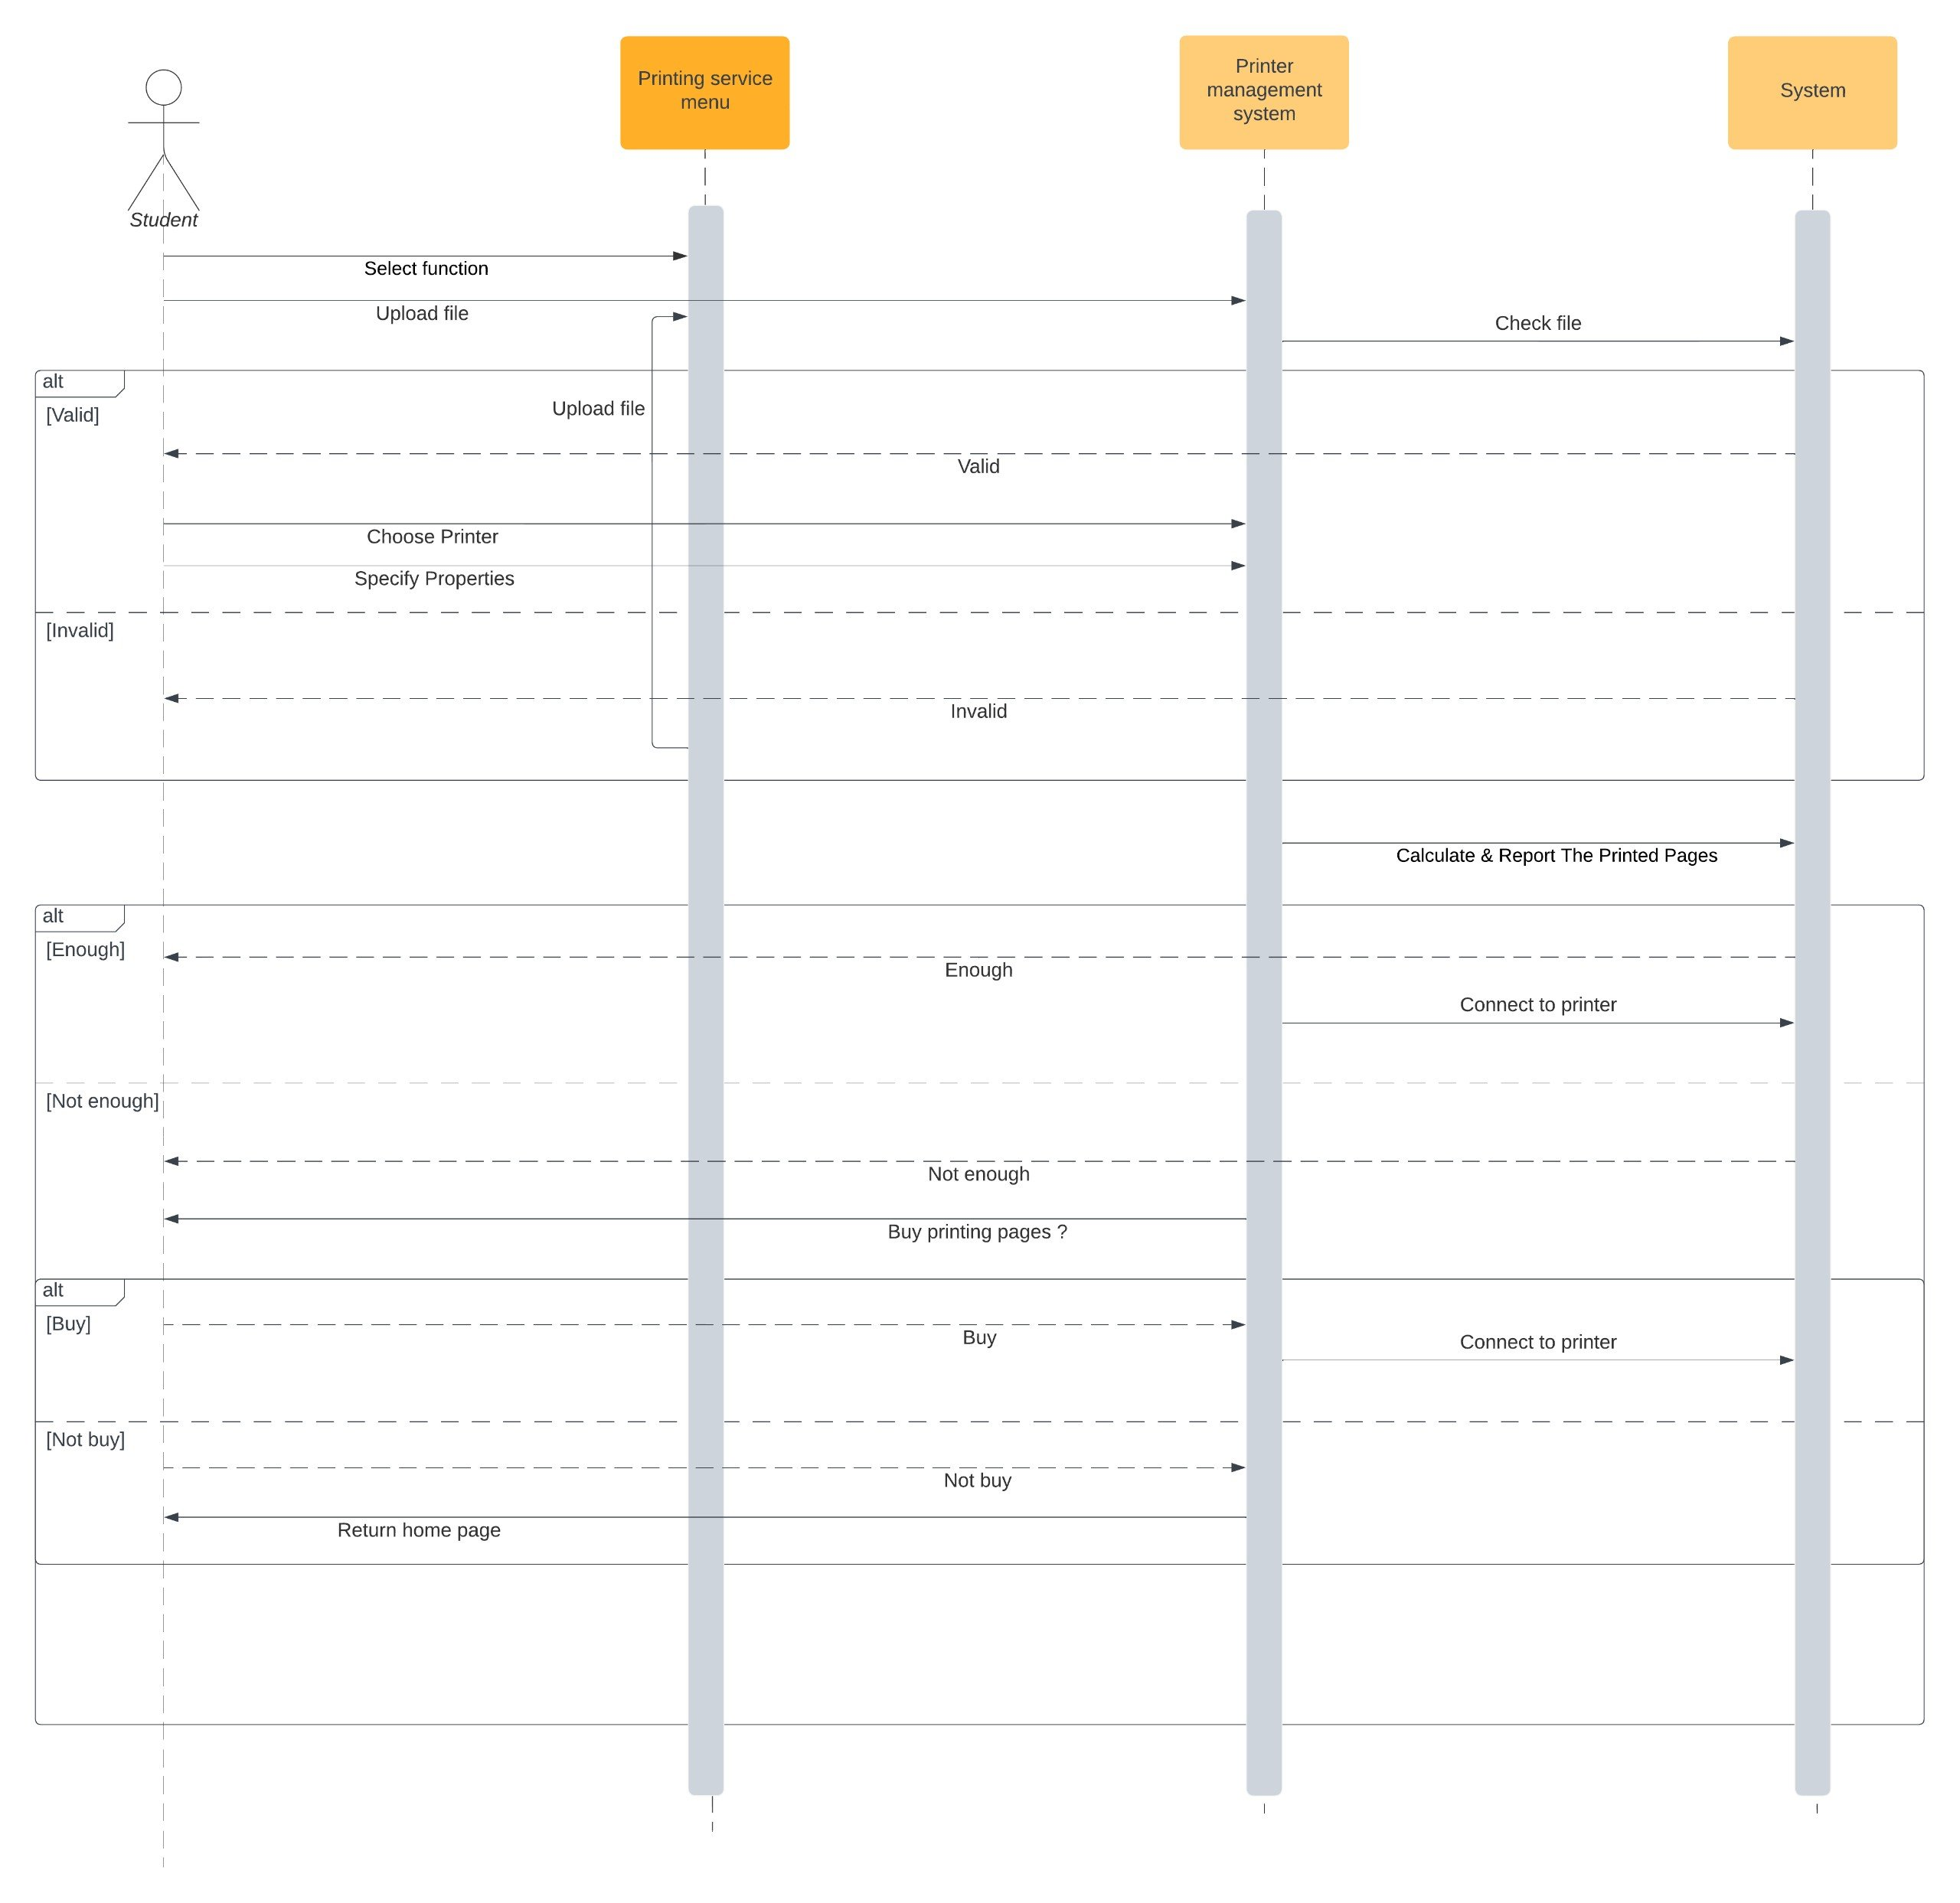
\includegraphics[scale=.19]{images/Task2/SequenceDiagrams/RequestForPrintingService.jpg}
    \end{center}
    \label{refhinh1}
    \end{figure}
    \end{center}

    \newpage
    \textbf{Mô tả:}
    \begin{itemize}
        \item Người dùng tiến hành tải file in lên hệ thống quản lý.
        \item Hệ thống sẽ tự động kiểm tra tính hợp lệ và hiển thị thông báo cho người dùng:
        \begin{itemize}
            \item Nếu file hợp lệ người dùng được phép chọn máy in và cấu hình các thuộc tính in.
            \item Nếu file không hợp lệ hệ thống đưa người dùng trở lại bước tải file ban đầu và tải lên lại file mới.
        \end{itemize}
        \item Tiếp đó hệ thống sẽ tính toán lại số lượng trang được in còn lại của sinh viên và báo cáo lại cho người dùng:
        \begin{itemize}
            \item Nếu đủ số trang hệ thống sẽ tiến hành in cho sinh viên.
            \item Nếu thiếu số trang để in người dùng được chuyển tới chức năng mua trang in:
            \begin{itemize}
                \item Nếu sinh viên mua đủ hoặc hơn số trang để in hệ thống sẽ tiến hành in.
                \item Nếu sinh viên chọn không mua hệ thống sẽ đem sinh viên về trang chủ
            \end{itemize}
        \end{itemize}
    \end{itemize}

    \newpage
    \subsubsection{Make Online Payment}
    \begin{center}
    \begin{figure}[!htp]
    \begin{center}
     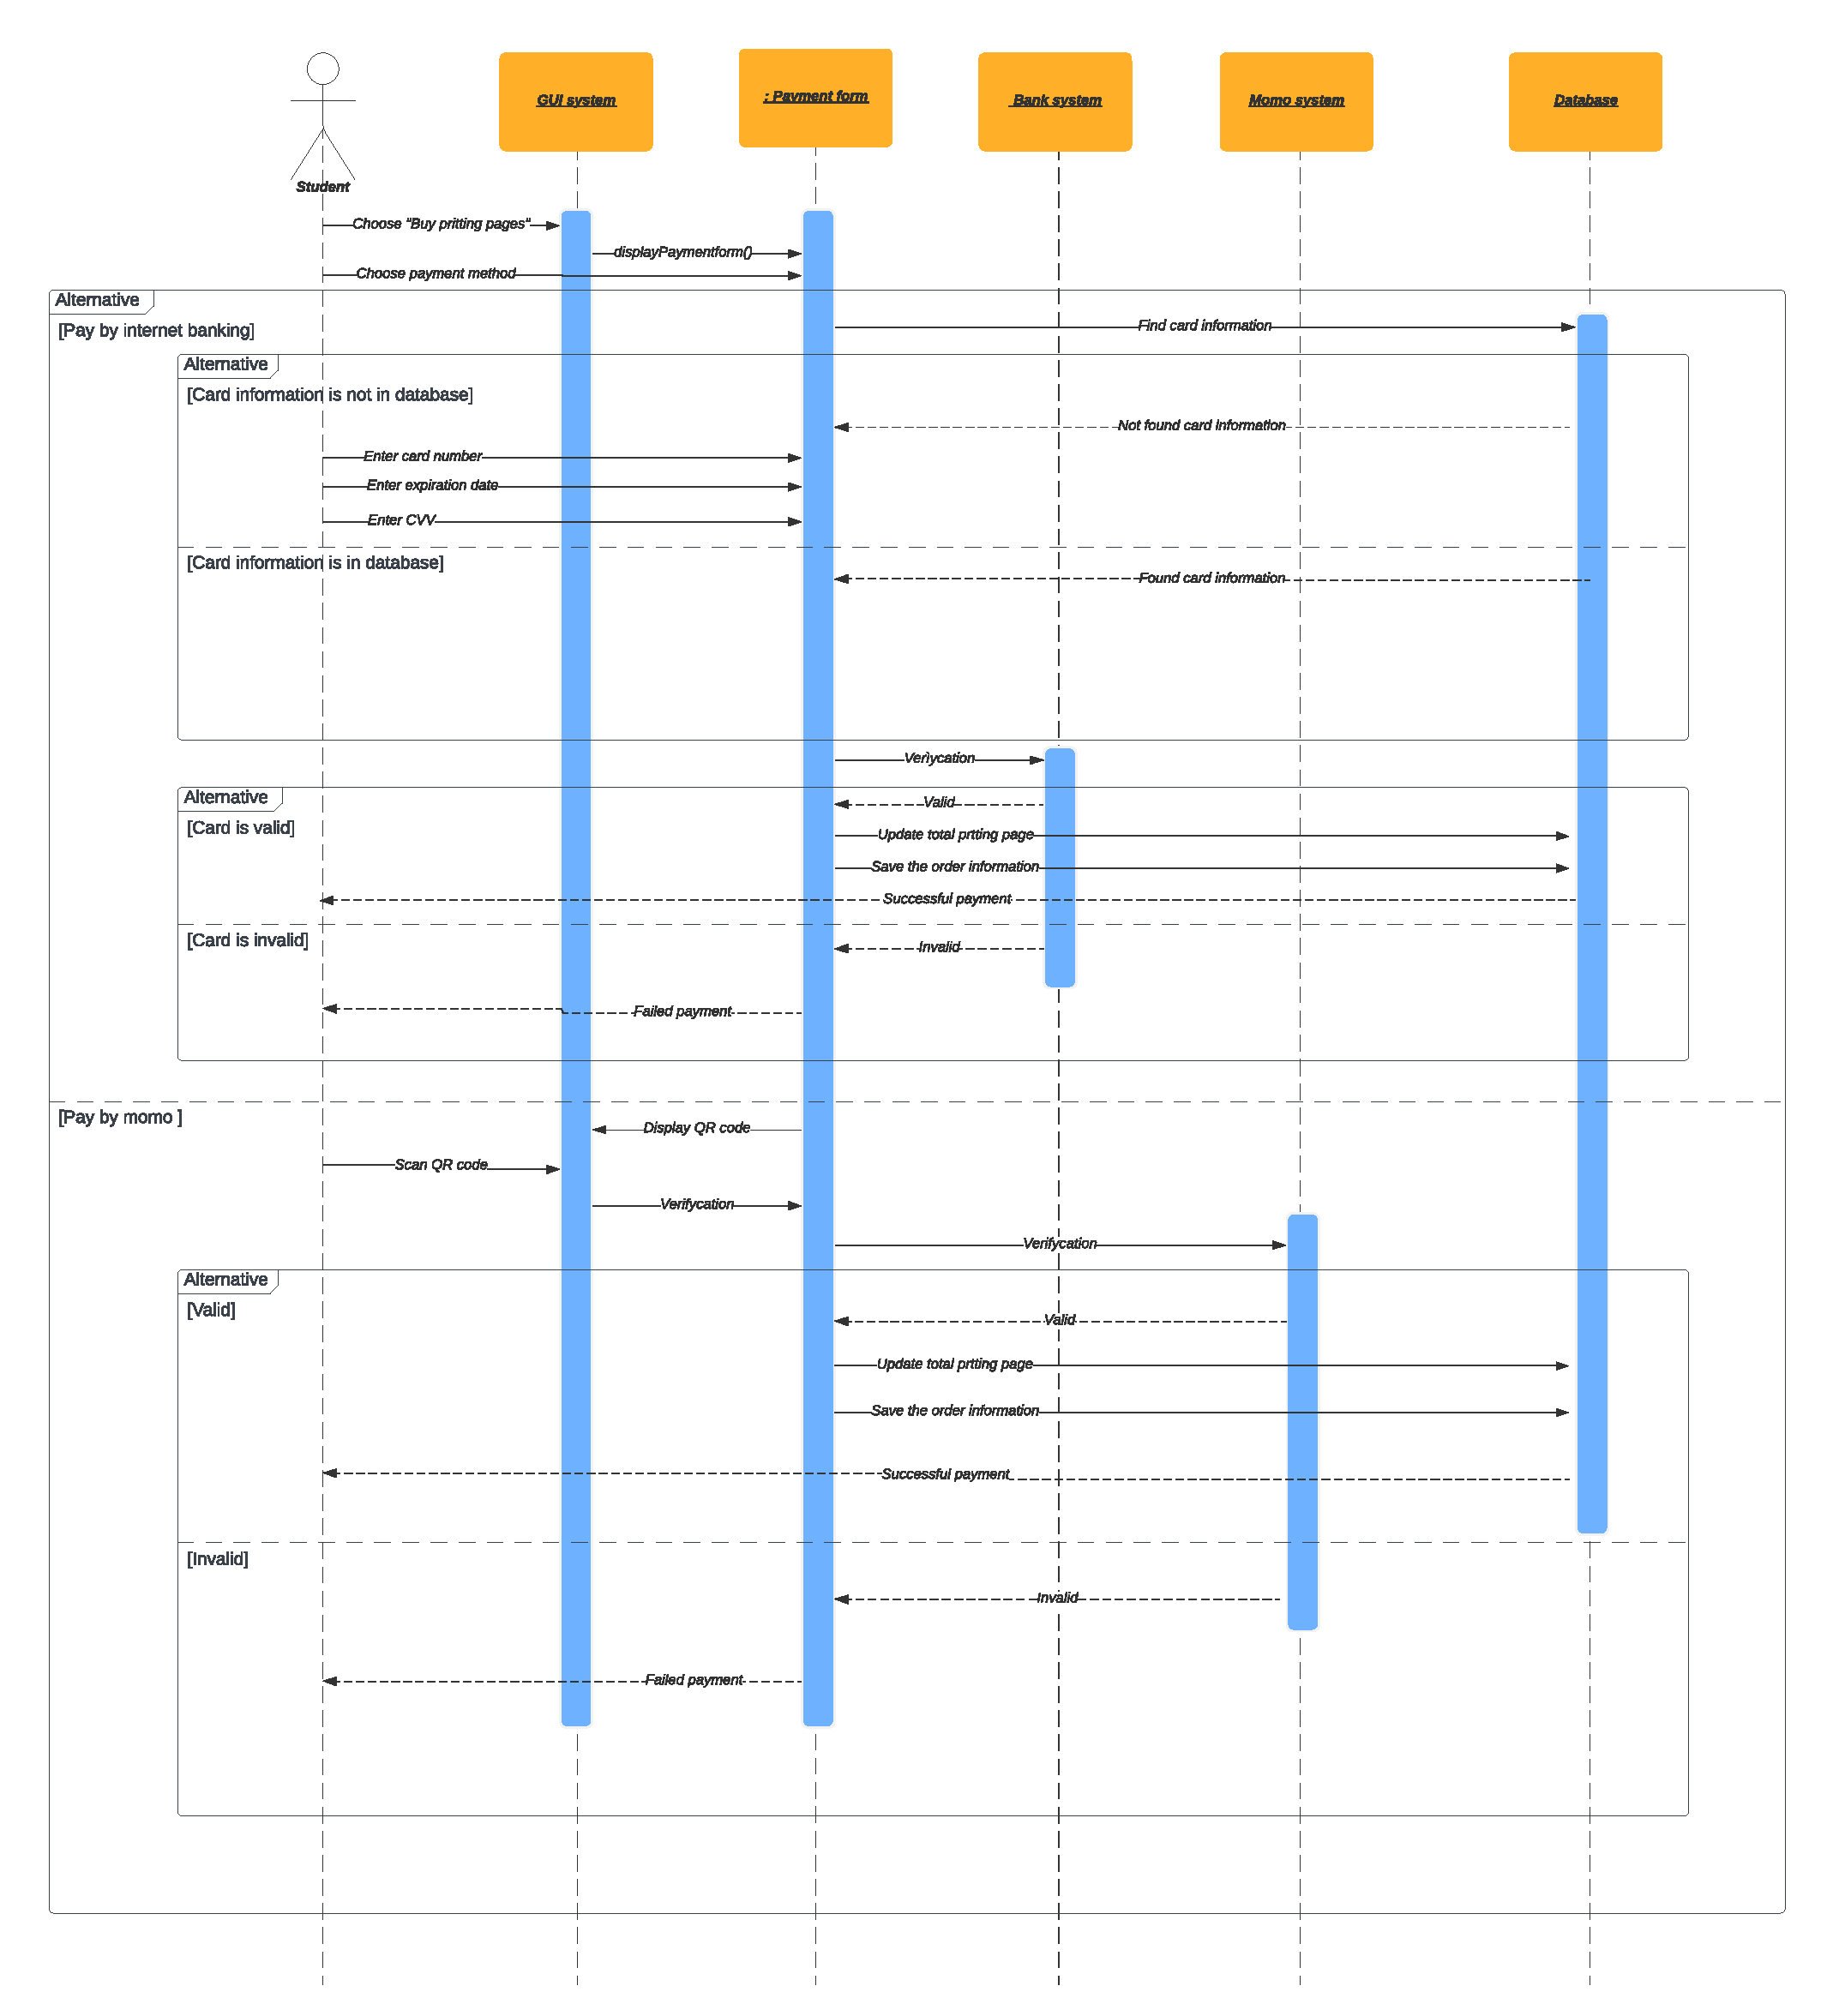
\includegraphics[scale=0.45]{images/Task2/SequenceDiagrams/PaymentSequence.pdf}
    \end{center}
    \label{refhinh1}
    \end{figure}
    \end{center}
        \newpage
    \textbf{Mô tả:}
\begin{itemize}
        \item Sinh viên chọn dịch vụ mua giấy in để tiến hành mua thêm giấy in
        \item Sau khi đăng nhập thành công, sinh viên chọn chức năng "Mua giấy in", sau đó hệ thống sẽ hiển thị giao diện mua giấy in để sinh viên có thể chọn số lượng giấy in mình cần mua.
        \item Hệ thống dựa vào số lượng giấy in mà sinh viên chọn cùng với giá của giấy in tại thời điểm sinh viên mua mà tính toán ra số tiền cần trả để sinh viên kiểm tra và xác nhận.
        \item Sau khi xác nhận giá thì sinh viên sẽ chọn 1 trong 2 phương thức thanh toán là qua visacard hay là ví điện tử momo
        \begin{itemize}
            \item Nếu sinh viên chọn thanh toán qua visacard thì cần phải nhập thông tin bao gốm số thẻ, ngày hết hạn và mã bảo vệ. Hệ thống sẽ gửi API đến ngân hàng để xác nhận thông tin thanh toán.
            \item Nếu sinh viên chọn thanh toán qua momo thì hệ thống sẽ hiển thị mã QR, sinh viên thực hiện quét mã và hệ thống sẽ gửi API đến ví điện tử momo để xác nhận thông tin thanh toán.
        \end{itemize}
        \item Trong cả 2 trường hợp nếu thanh toán thành công thì sẽ cập nhật số lượng giấy in của sinh viên, lưu lại hóa đơn thanh toán đồng thời hiển thị ra màn hình để sinh viên xác nhận.
        \item Nếu việc thanh toán thất bại thì hệ thống sẽ hiển thị thông báo lỗi và quay trở về bước thanh toán trước đó.
    \end{itemize}


    \newpage
    \subsubsection{Manage Printers}
    \begin{center}
    \begin{figure}[!htp]
    \begin{center}
     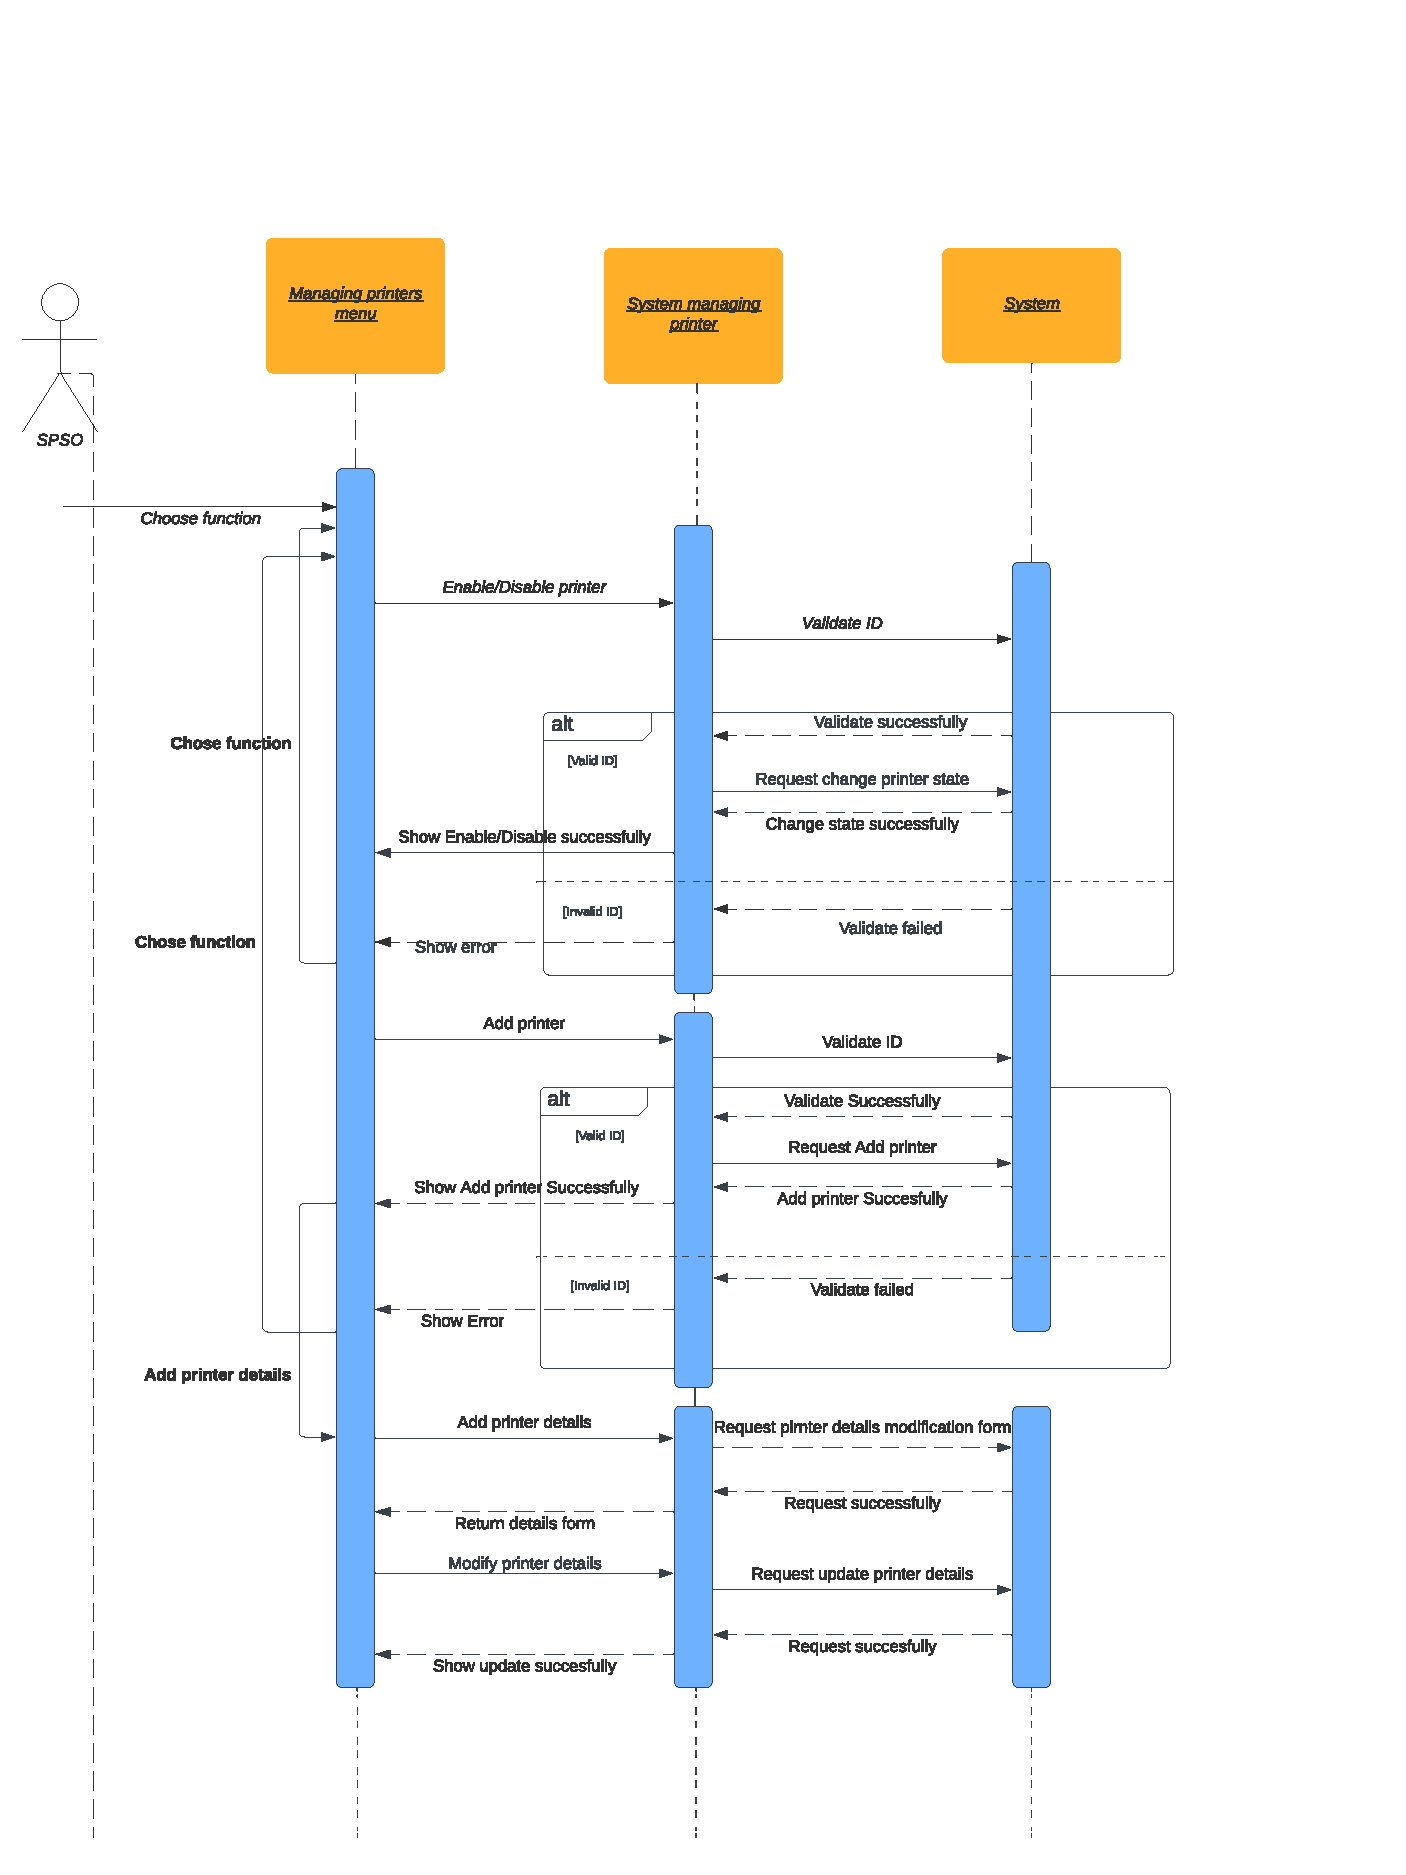
\includegraphics[scale=.6]{images/Task2/SequenceDiagrams/ManagePrinter.pdf}
    \end{center}
    \label{refhinh1}
    \end{figure}
    \end{center}

    \textbf{Mô tả:}
    Sau khi đăng nhập, SPSO sẽ vào giao diện để dành riêng cho SPSO, sau đó SPSO có thể chọn vào Quản lý máy in. \\

    Tại trang quản lý máy in, SPSO có thể lựa chọn giữa chức năng Thêm máy in và Bật / Tắt máy in. 
    \begin{itemize}
        \item Sau khi chọn Bật / Tắt máy in, SPSO nhập ID cho máy in cần bật hoặc tắt. Nếu ID hợp lệ, hệ thống quản lý máy in sẽ gửi request cho hệ thống in ấn để thay đổi trạng thái máy in theo yêu cầu, rồi trả về thống báo đã thay đổi cho SPSO. Nếu nhập sai ID hoặc ID không hợp lệ thì hệ thống sẽ báo lỗi sai ID và trả SPSO về trang quản lý máy in.
        \item Nếu chọn thêm máy in, SPSO nhập ID cho máy in muốn được thêm mới. Nếu ID hợp lệ, hệ thống quản lý máy in sẽ gửi request cho hệ thống in ấn để cho phép SPSO nhập tiếp các thông tin còn lại của máy in (tên, mẫu mã, ...) rồi gửi các thông tin đó đến hệ thống. Sau đó, hệ thống sẽ cập nhật thông tin máy in giống như đã nhập và trả về thống báo đã thêm thành công.
    \end{itemize}


    \newpage
    \subsubsection{Configure System}
    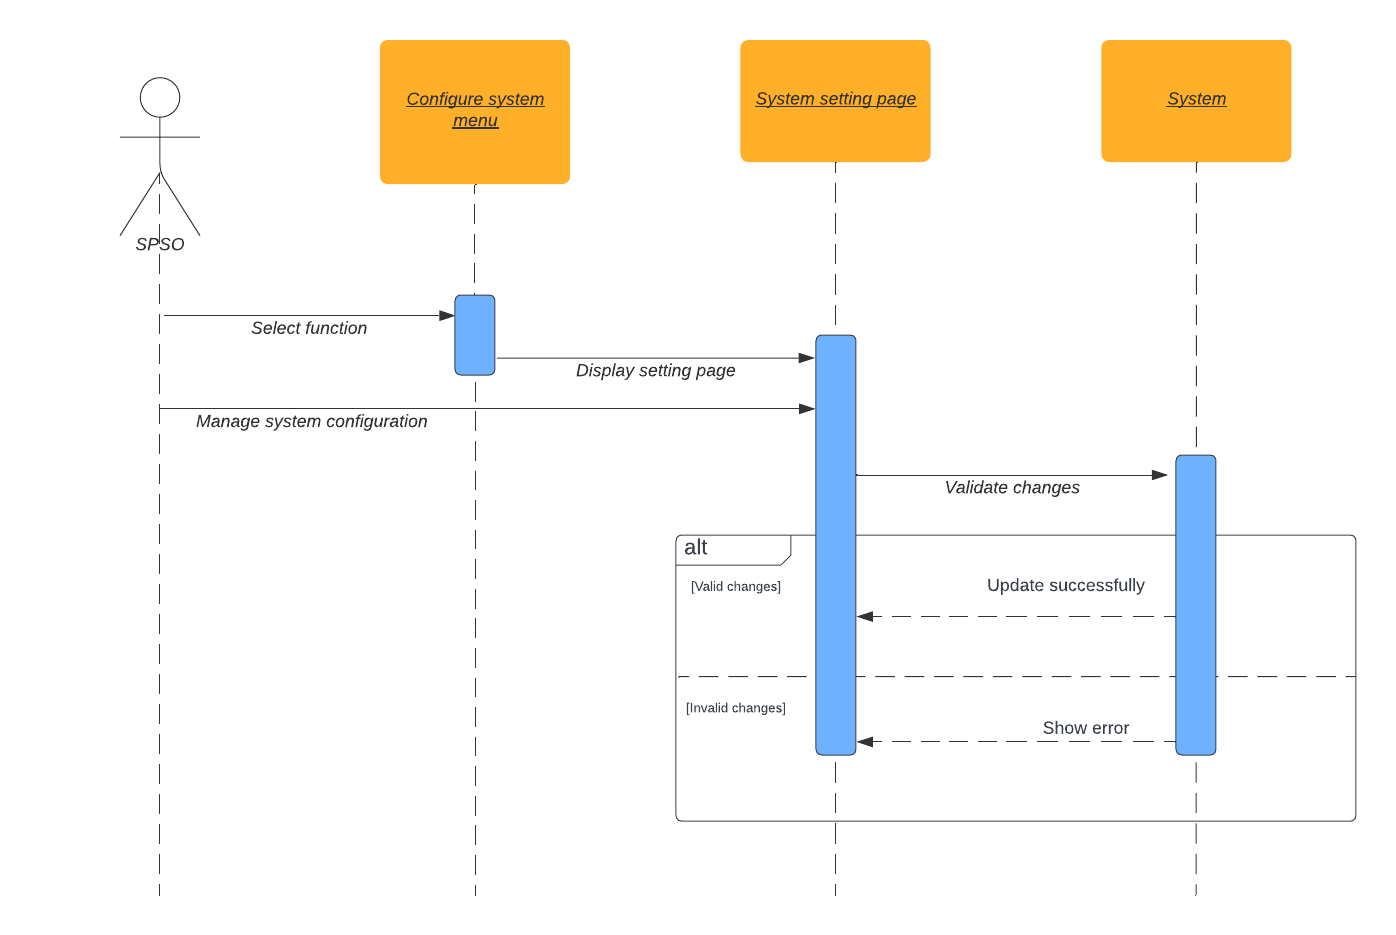
\includegraphics[width=\textwidth]{images/Task2/SequenceDiagrams/ConfigureSystem_SequenceDiagram.png}
    \textbf{Mô tả:}
    Biểu đồ mô tả sự tương tác của SPSO với các objects khác là Configure system menu, System setting page và system. Vai trò của SPSO là chọn chức năng cần tùy chỉnh trong Configure system menu và tiến hành tùy chỉnh trong system setting page. Nhìn qua biểu đồ, ta có thể thấy thời gian hoạt động của System setting page là nhiều nhất, đúng với vai trò chính của chức năng tùy chỉnh cấu hình hệ thống.\\

    \newpage
    \subsubsection{Log In}
    \begin{center}
    \begin{figure}[!htp]
    \begin{center}
     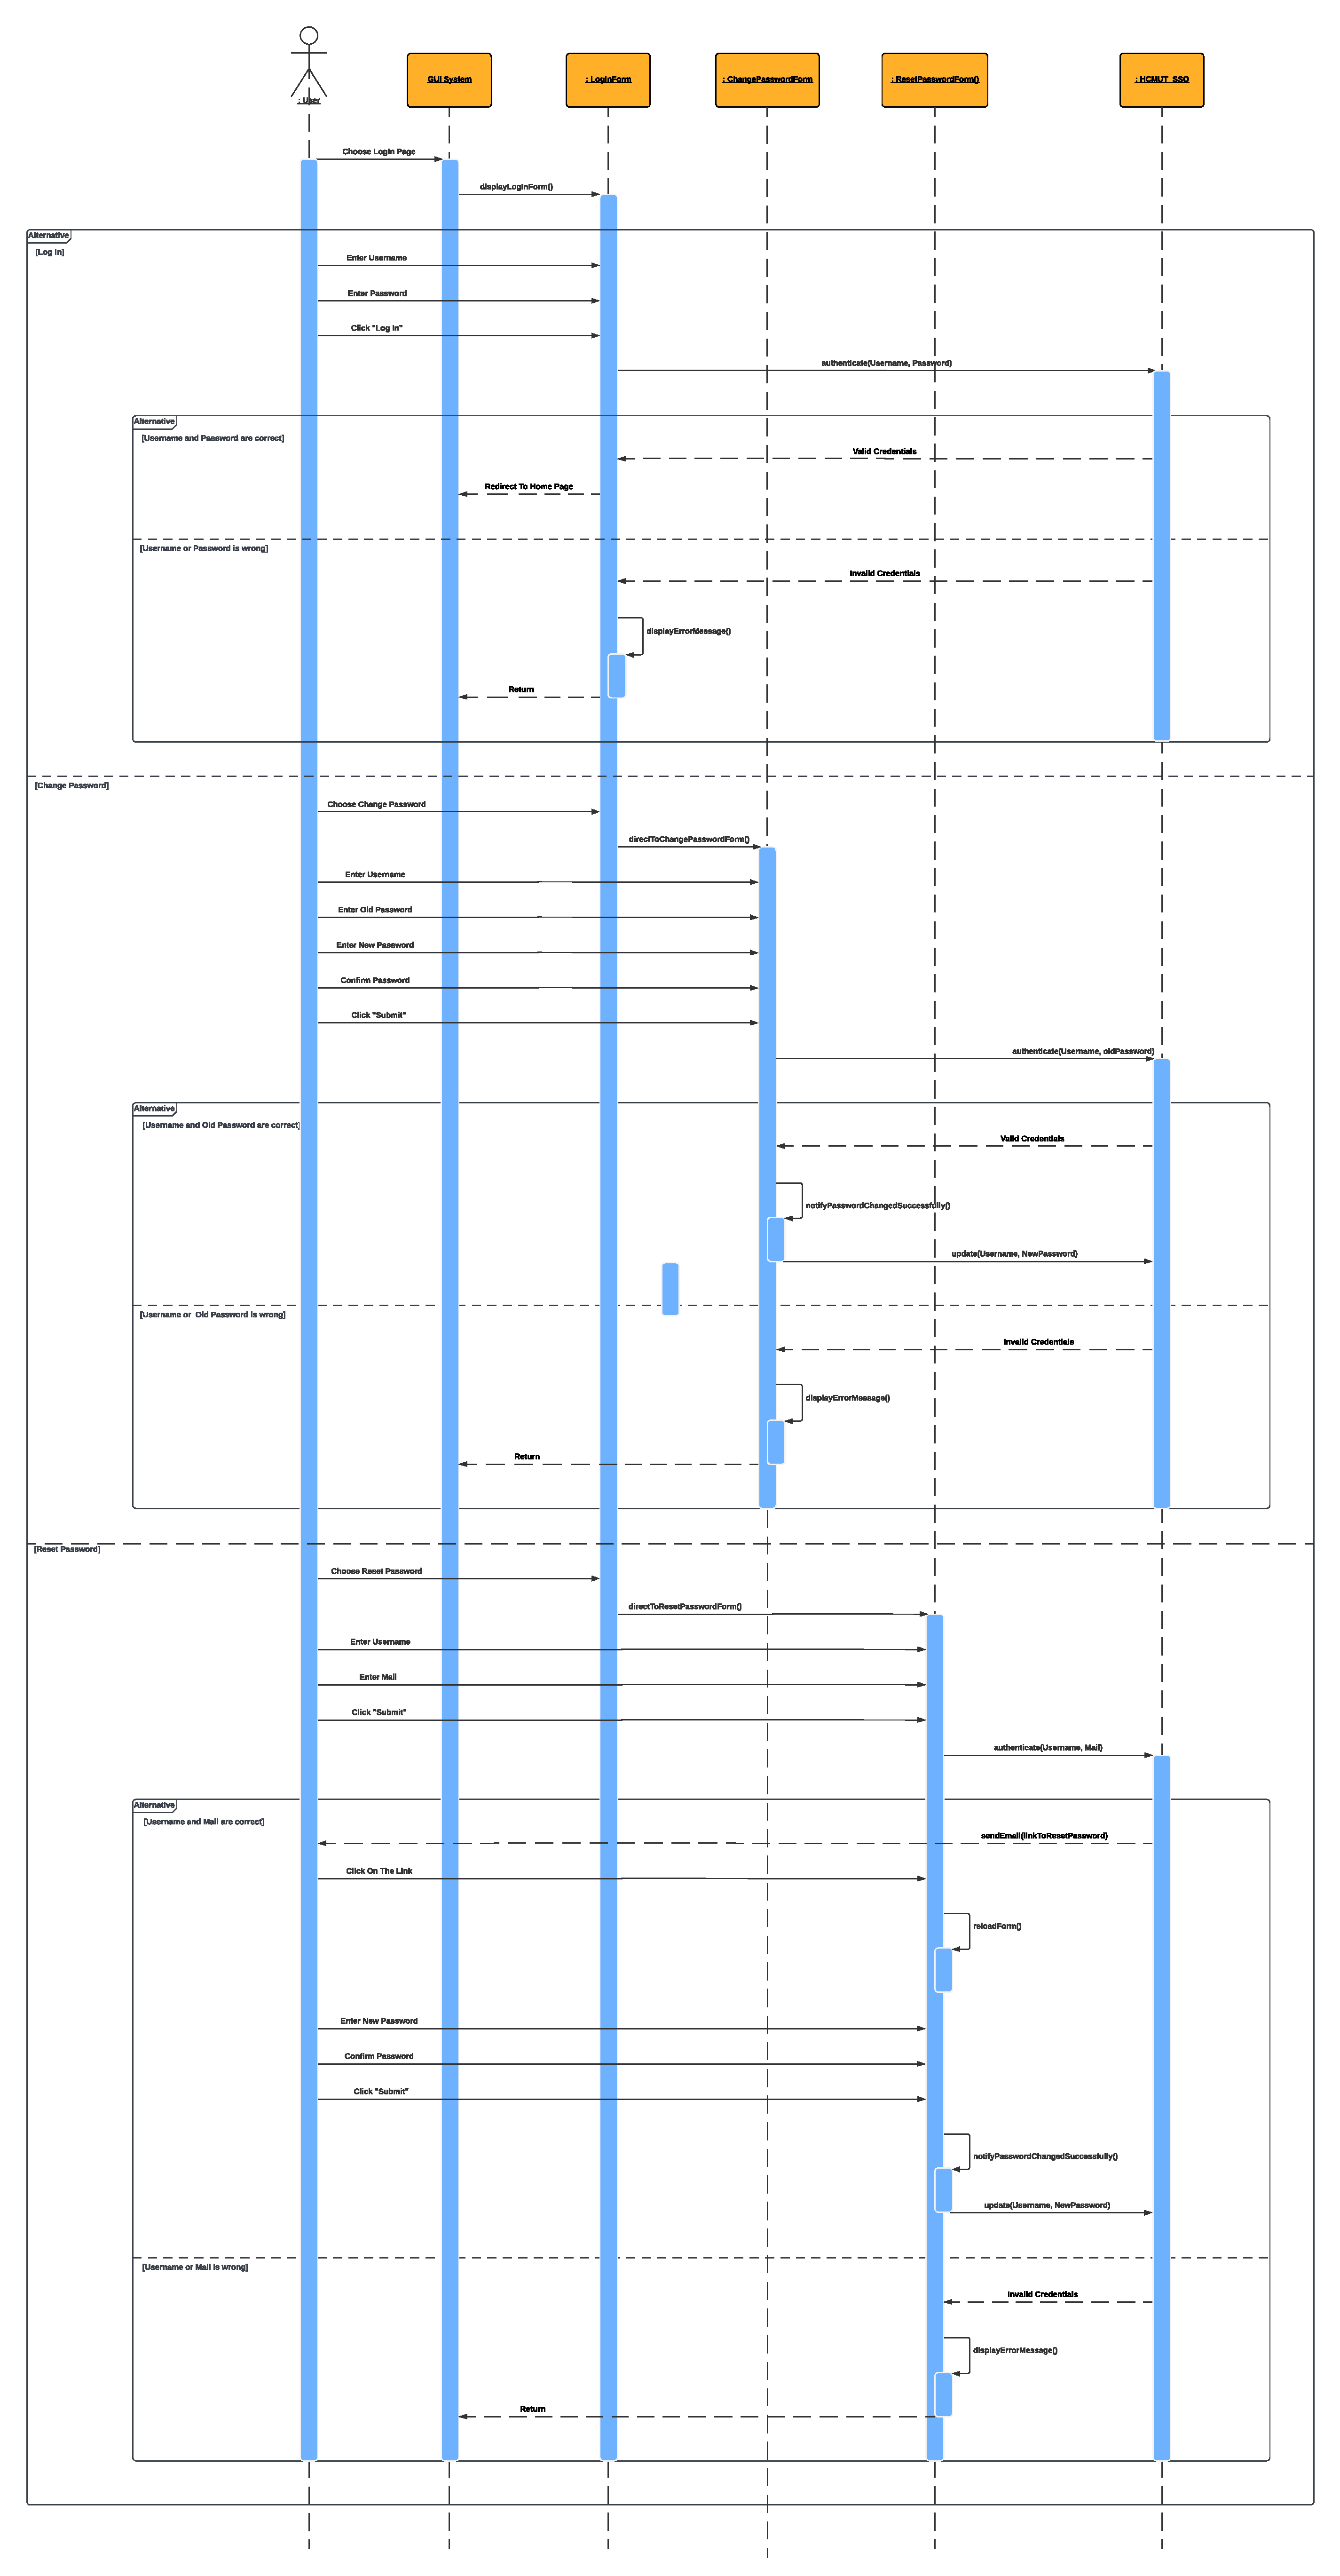
\includegraphics[scale=.21]{images/Task2/SequenceDiagrams/LogIn.pdf}
    \end{center}
    \label{refhinh1}
    \end{figure}
    \end{center}

    \textbf{Mô tả:}\\
    
        Tại giao diện đăng nhập, người dùng nhập thông tin (username, password) và chọn "Log In" để gửi yêu cầu đăng nhập.\\
        
        Dịch vụ xác thực HCMUT\_SSO sẽ tiến hành xác thực thông tin đăng nhập mà người dùng cung cấp.
        \begin{itemize}
            \item Thông tin xác thực hợp lệ: Người dùng sẽ được điều hướng tới giao diện trang chủ của trang web để tiếp tục sử dụng các dịch vụ khác.
            \item Thông tin xác thực không hợp lệ: Tại giao diện đăng nhập, một thông báo về sai thông tin đăng nhập sẽ được hiển thị.
        \end{itemize}
        
        Tại giao diện đăng nhập, người dùng còn có 2 tuỳ chọn khác:
        \begin{itemize}
            \item Thay đổi mật khẩu: 
            \begin{itemize}
                \item Khi người dùng chọn "Change Password", trang web sẽ điều hướng tới trang Change Password. Tại đây người dùng cần cung cấp các thông tin (username, old password, new password, comfirm password) và chọn "Submit" để gửi yêu cầu thay đổi mật khẩu.
                \item Dịch vụ xác thực HCMUT\_SSO sẽ tiến hành xác thực thông tin đăng nhập mà người dùng cung cấp:
                \begin{itemize}
                    \item Thông tin xác thực hợp lệ: Mật khẩu mới sẽ được cập nhật. Tại giao diện thay đổi mật khẩu, một thông báo về việc thay đổi mật khẩu thành công sẽ được hiển thị.
                    \item Thông tin xác thực không hợp lệ: Tại giao diện thay đổi mật khẩu, một thông báo về việc thay đổi mật khẩu thất bại sẽ được hiển thị.
                \end{itemize}
            \end{itemize}
            \item Quên mật khẩu:
            \begin{itemize}
                \item Khi người dùng chọn "Reset Password", trang web sẽ điều hướng tới trang Reset Password. Tại đây người dùng cần cung cấp các thông tin (username, email) và chọn "Submit" để gửi yêu cầu đặt lại mật khẩu.
                \item Dịch vụ xác thực HCMUT\_SSO sẽ tiến hành xác thực thông tin mà người dùng cung cấp:
                \begin{itemize}
                    \item Thông tin xác thực hợp lệ: Dịch vụ xác thực sẽ tiến hành gửi một "link" xác nhận yêu cầu đặt lại mật khẩu thông qua email mà người dùng cung cấp. Người dùng cần truy cập "link" này, sau đó cung cấp thông tin (new password, confirm password) và chọn "submit" để gửi yêu cầu đặt lại mật khẩu. Khi đó, mật khẩu mới sẽ được cập nhật. Tại giao diện đặt lại mật khẩu, một thông báo về việc đặt lại mật khẩu thành công sẽ được hiển thị.
                    \item Thông tin xác thực không hợp lệ: Tại giao diện đặt lại mật khẩu, một thông báo về sai thông tin tài khoản sẽ được hiển thị.
                \end{itemize}
            \end{itemize}
        \end{itemize}